\chapter{Implementation and Evaluation}
\label{chap:implementation}

This chapter turns the design of Chapter~\ref{chap:methodology} into running code and reports the empirical evaluation. It begins with the technology stack and the layout of the project tree, drills into the four engineering subsystems that carry most of the platform's risk --- the transfer engine, the per-currency partner-saldo subsystem, the offline behaviour and the design system --- and closes with the testing strategy, the performance measurements, the user-acceptance trial and an honest account of the limitations that remain.

\section{Technology Stack and Project Structure}
\label{sec:stack}

The implementation rests on a deliberately narrow stack. On the client the platform uses Flutter 3 with Dart 3, the BLoC library (\texttt{flutter\_bloc}~9.x) for state management, \texttt{get\_it} with \texttt{injectable} for dependency injection, \texttt{go\_router} for navigation, \texttt{hive} for a small local cache (used only for read-side resilience --- see section~\ref{sec:offline}), \texttt{trina\_grid} for desktop data grids, and \texttt{lucide\_icons\_flutter} wrapped by an internal \texttt{AppIcons} facade. On the server the platform uses Supabase --- managed PostgreSQL~16, GoTrue for authentication, PostgREST and a thin RPC layer for direct stored-procedure calls, Realtime for logical-replication subscriptions, and Storage. The complete dependency list is reproduced in Table~\ref{tab:stack}.

{\singlespacing
\begin{table}[h]
  \caption{Technology stack of the implementation}
  \label{tab:stack}
  \centering
  \begin{tabular}{lll}
    \toprule
    \textbf{Layer}        & \textbf{Technology}                       & \textbf{Version}\\
    \midrule
    Language              & Dart                                      & 3.x\\
    UI framework          & Flutter                                   & 3.x stable\\
    State management      & flutter\_bloc                             & 9.x\\
    Dependency injection  & get\_it + injectable                      & 8.x / 2.x\\
    Routing               & go\_router                                & 15.x\\
    Local cache           & hive + hive\_flutter                      & 2.x / 1.x\\
    Code generation       & freezed + json\_serializable              & 3.x / 6.x\\
    Iconography           & lucide\_icons\_flutter + AppIcons facade  & 0.5\\
    Desktop grids         & trina\_grid                               & 1.x\\
    Charts                & fl\_chart                                 & 0.70\\
    Backend               & Supabase (PostgreSQL\,16 + Realtime)      & latest stable\\
    Tests                 & flutter\_test, bloc\_test, mocktail       & latest\\
    \bottomrule
  \end{tabular}
\end{table}
}

The source tree (Listing~\ref{lst:tree}, abridged) follows the Clean-Architecture layering of section~\ref{sec:cleanarch2}. Each top-level directory under \texttt{lib/} maps to a single layer; each presentation feature has its own folder with three sub-folders for BLoC, pages and widgets.

\begin{lstlisting}[caption={Source tree (abridged)},label={lst:tree}]
lib/
  app.dart                       # MaterialApp + theming
  main.dart                      # Bootstrap, DI, Supabase init
  core/
    constants/                   # Currency tier map, role enum
    di/                          # get_it configuration
    icons/                       # AppIcons facade
    network/                     # Connectivity probe
    routing/                     # GoRouter table
    services/                    # Cross-cutting services
    supabase/                    # Typed Supabase client
    theme/                       # Dark-fintech palette
    utils/                       # Money, currency helpers
  domain/
    entities/                    # Pure-Dart entities
    repositories/                # Abstract interfaces
    services/                    # Pure-Dart domain services
    usecases/                    # Use case classes
  data/
    datasources/remote/          # SupabaseTransfersDataSource, ...
    repositories/                # Repository implementations
    services/                    # Data-layer services
  presentation/
    auth/                        # Authentication
    dashboard/                   # Branch / per-currency totals
    transfers/                   # Transfer creation, list, attach
    counterparties/              # Partner cards, attach flows
    clients/                     # Client list, wallet
    branches/                    # Branch admin
    users/                       # User admin
    reports/                     # Per-currency reconciliation
    analytics/                   # Charts
    notifications/               # Real-time inbox
    admin/                       # Director approval queue
    settings/                    # Preferences
    common/widgets/              # Shared widgets
supabase/migrations/             # 66 numbered .sql files
\end{lstlisting}

The dependency-injection container is initialised once at startup. It registers the Supabase client as a singleton, then registers a remote data source per domain area, then a repository per area on top of it. The BLoC layer pulls its repositories from this container, which keeps every BLoC ignorant of how the data layer is wired.

\section{The Transfer Engine: Idempotency and Atomicity}
\label{sec:transfer}

The transfer creation procedure is the most safety-critical part of the system. The client side issues a transfer-creation request that carries an idempotency key (a UUID generated in the initialiser of the form widget, before the user has a chance to tap \emph{Submit} twice). Listing~\ref{lst:submit} shows the BLoC code path.

\begin{lstlisting}[language=Java,caption={Submitting a transfer (Dart, BLoC)},label={lst:submit}]
class TransfersBloc extends Bloc<TransfersEvent, TransfersState> {
  TransfersBloc(this._repo) : super(const TransfersState.idle()) {
    on<SubmitTransfer>(_onSubmit);
  }

  Future<void> _onSubmit(
      SubmitTransfer event, Emitter<TransfersState> emit) async {
    emit(const TransfersState.submitting());
    final result = await _repo.createTransfer(
      branchId: event.branchId,
      srcAccountId: event.srcAccountId,
      dstAccountId: event.dstAccountId,
      srcAmount: event.srcAmount,
      dstAmount: event.dstAmount,
      rate: event.rate,
      viaCounterpartyId: event.viaCounterpartyId,
      idempotencyKey: event.idempotencyKey, // UUID v4 from form init
    );
    result.fold(
      (failure) => emit(TransfersState.error(failure.toReadableMessage())),
      (transfer) => emit(TransfersState.created(transfer)),
    );
  }
}
\end{lstlisting}

The server side wraps the entire creation procedure in a single PL/pgSQL stored function with \texttt{SECURITY DEFINER}, which guarantees that all subordinate operations execute inside the same implicit transaction. Listing~\ref{lst:rpc} shows an abridged form of the procedure. The function validates the inputs, picks the next sequential transaction code, inserts the row into \texttt{transfers}, updates \texttt{branch\_accounts}, inserts the matching ledger entries, optionally records a counterparty transaction and a commission row, and writes an audit-log entry. Any failure raises an exception, which rolls back the whole transaction.

\begin{lstlisting}[language=SQL,caption={Stored procedure: create\_transfer (abridged)},label={lst:rpc}]
CREATE OR REPLACE FUNCTION create_transfer(
  p_idempotency_key  UUID,
  p_branch_id        UUID,
  p_src_account_id   UUID,
  p_dst_account_id   UUID,
  p_via_cp_id        UUID,
  p_src_amount       NUMERIC,
  p_dst_amount       NUMERIC,
  p_rate             NUMERIC
) RETURNS UUID
LANGUAGE plpgsql AS $$
DECLARE
  v_existing UUID;
  v_transfer UUID;
  v_actor    UUID := auth.uid();
BEGIN
  -- Short-circuit on duplicate
  SELECT id INTO v_existing FROM transfers
   WHERE idempotency_key = p_idempotency_key;
  IF FOUND THEN RETURN v_existing; END IF;

  -- Role and branch authorisation
  PERFORM assert_can_write_branch(v_actor, p_branch_id);

  -- Atomic value movement
  INSERT INTO transfers (...) VALUES (...) RETURNING id INTO v_transfer;
  UPDATE branch_accounts SET balance = balance - p_src_amount
   WHERE id = p_src_account_id;
  IF p_dst_account_id IS NOT NULL THEN
    UPDATE branch_accounts SET balance = balance + p_dst_amount
     WHERE id = p_dst_account_id;
  END IF;
  INSERT INTO ledger_entries (...) VALUES (...);   -- credit on source
  INSERT INTO ledger_entries (...) VALUES (...);   -- debit on destination

  -- Partner-mediated branch: adjust per-currency saldo
  IF p_via_cp_id IS NOT NULL THEN
    INSERT INTO counterparty_transactions (...) VALUES (...);
    PERFORM bump_saldo(p_via_cp_id,
                       p_dst_currency,
                       p_dst_amount);
  END IF;

  PERFORM audit('transfer', v_transfer, 'create', v_actor);
  RETURN v_transfer;
END $$;
\end{lstlisting}

The properties the function gives in exchange for its size are worth stating explicitly. Atomicity is structural: every subordinate operation executes inside the same transaction, so either all succeed or none take effect. Idempotency is structural too: the UNIQUE partial index on \texttt{idempotency\_key} ensures that a second call with the same key short-circuits at the first lookup and returns the original transfer ID. Authorisation is double-belt-and-braces: even though Row-Level Security would block an unauthorised client, the \texttt{assert\_can\_write\_branch} call raises a loud exception, which surfaces in monitoring and is easier to debug than silent zero-row writes. The complexity per call is $O(1)$: a handful of indexed lookups and a handful of inserts.

\section{Partner Operations and Per-Currency Saldo}
\label{sec:partner}

Partner-mediated transfers are exposed in three places in the user interface. The first is the regular transfer-creation form, which has an optional \emph{via partner} field; selecting a partner here switches the form into partner-mediated mode and adds the partner-saldo preview block. The second is an \emph{attach} dialog reached from an existing transfer in the list, which converts an already-created own-branch transfer into a partner-mediated one without altering the value movement on the operator's side. The third is the symmetric \emph{attach a transfer} dialog reached from the partner card, which lists unattached transfers and lets the operator pick one. All three surfaces share a single \texttt{DealerRatesBlock} widget and a single \texttt{PartnerSaldoPreview} widget --- the design pressure to reuse them came from a real episode in which two separately written copies of the preview drifted apart on a corner case involving negative saldo, and the divergence was caught only at the operator's screen.

The per-currency saldo update is the operationally novel piece. A naive earlier iteration of the schema collapsed every partner debt into US dollars at the dealer-mode buy rate, on the assumption that the operator would treat the dollar saldo as the canonical view. That assumption broke down in practice: the same partner routinely received payouts in Russian roubles, Turkish liras and Uzbek som on the same day, and the dollar-collapsed view masked an exposure to each individual currency that the operator wanted to see. Migration~047 of the production schema replaced the collapsed model with the per-currency JSONB attribute described in section~\ref{sec:domainmodel}. The dealer-mode spread, which the collapsed model had hidden in the FX-difference account, was moved to a dedicated \texttt{spread\_profit} column on \texttt{transfers}, where it could be queried and totalled independently. Listing~\ref{lst:bump} shows the \texttt{bump\_saldo} helper used inside \texttt{create\_transfer}.

\begin{lstlisting}[language=SQL,caption={Per-currency saldo update (PL/pgSQL)},label={lst:bump}]
CREATE OR REPLACE FUNCTION bump_saldo(
  p_cp_id    UUID,
  p_currency TEXT,
  p_delta    NUMERIC
) RETURNS void
LANGUAGE plpgsql AS $$
BEGIN
  UPDATE counterparties
     SET saldo_by_currency =
           jsonb_set(
             saldo_by_currency,
             ARRAY[p_currency],
             to_jsonb(
               COALESCE((saldo_by_currency->>p_currency)::NUMERIC, 0)
               + p_delta
             )
           )
   WHERE id = p_cp_id;
END $$;
\end{lstlisting}

The rounding rule applied to saldo updates was the source of a small but instructive iteration of its own. Round-half-up produced an asymmetric drift over long sequences of transfers; banker's rounding (round half to even) eliminated it. The decision is recorded in migration~056 and is referenced from the \texttt{round\_partner\_amount} helper used inside \texttt{bump\_saldo}.

\section{The Approval Workflow in Code}
\label{sec:approvalimpl}

The Director-mediated approval workflow of section~\ref{sec:approval} is realised by three stored procedures and one screen. The \texttt{request\_approval} RPC accepts the entity type, the target row's ID, the proposed change as a JSONB diff and the snapshot of the current row state (collected client-side from the BLoC's last known State and validated against a fresh SELECT inside the procedure). Listing~\ref{lst:request} shows the principal columns of the resulting row.

\begin{lstlisting}[language=SQL,caption={Pending approval: principal columns},label={lst:request}]
CREATE TABLE pending_approvals (
  id              UUID PRIMARY KEY DEFAULT gen_random_uuid(),
  branch_id       UUID NOT NULL REFERENCES branches(id),
  entity          TEXT NOT NULL,
  entity_id       UUID NOT NULL,
  proposed_change JSONB NOT NULL,
  before_snapshot JSONB NOT NULL,
  status          TEXT NOT NULL DEFAULT 'requested',
  requested_by    UUID NOT NULL REFERENCES users(id),
  requested_at    TIMESTAMPTZ NOT NULL DEFAULT now(),
  resolved_by     UUID REFERENCES users(id),
  resolved_at     TIMESTAMPTZ
);
\end{lstlisting}

The matching \texttt{approve} RPC re-checks that the resolver's role is Director or Creator, applies the proposed change to the target row inside a transaction, writes the audit-log entry and marks the approval as resolved. Crucially, \texttt{approve} compares the current state of the target row with the captured snapshot and raises an exception if they differ; this catches the rare but real case in which the row was concurrently modified between the request and the approval. The Director's screen, illustrated in Figure~\ref{fig:approvalscreen}, renders the before and after states side by side with the changed columns highlighted.

\begin{figure}[h]
  \centering
  \begin{tikzpicture}[
    panel/.style={draw, rounded corners, fill=blue!5, minimum width=5cm, minimum height=2.6cm, font=\small, align=left, text width=4.6cm},
    btn/.style={draw, rounded corners, fill=blue!20, minimum width=2cm, minimum height=0.7cm, font=\small},
    btnRed/.style={draw, rounded corners, fill=red!15, minimum width=2cm, minimum height=0.7cm, font=\small},
    >=Stealth
  ]
    \node[panel] (before) at (0,0)  {\textbf{Before}\\\\ID: T-2156\\Dst currency: USD\\Dst amount: 540\\Rate: 0.94};
    \node[panel] (after) at (6,0)   {\textbf{After (proposed)}\\\\ID: T-2156\\\textbf{Dst currency: EUR}\\\textbf{Dst amount: 510}\\\textbf{Rate: 1.00}};
    \node[btn]   (apv)  at (3,-2)   {Approve};
    \node[btnRed] (rej) at (3,-3)   {Reject};
  \end{tikzpicture}
  \caption{Sketch of the Director's approval screen: before-state and proposed after-state shown side by side, changed columns in bold.}
  \label{fig:approvalscreen}
\end{figure}

\section{Offline Behaviour and Real-Time Updates}
\label{sec:offline}

Real-time updates are provided by Supabase Realtime, which streams logical-replication events to subscribed clients. The relevant BLoCs subscribe at startup to a small set of tables --- \texttt{transfers}, \texttt{pending\_approvals}, \texttt{notifications}, \texttt{branch\_accounts}; when an inbound event arrives, the BLoC reconciles its local list with the incoming row state and emits a refreshed State.

For offline tolerance the BLoC keeps the last successful list in memory (and, for the dashboard, in a small Hive box), so the operator can continue \emph{reading} their data when the network drops. \emph{Writes} are deliberately refused with a clearly worded error rather than queued for later replay. The decision deserves a short justification, because it goes against the dominant prejudice in the offline-first literature. The financial semantics of the platform make a refused write strictly safer than a write replayed out of order: a refused write does not produce a row in \texttt{transfers}, the operator sees a banner and tries again when the connection is back, and the partner saldo never moves into an inconsistent state. A replayed write, by contrast, could land after a subsequent change had already been recorded against the same accounts, producing a balance that depends on replay order rather than on intent. The platform errs on the safer side. An asynchronous write queue with strong ordering guarantees is named in the future-work section of the Conclusions.

\section{UI/UX Design Language}
\label{sec:design}

The visual language is a dark-fintech palette built around a saturated mint primary (\texttt{\#00D1A0}), a softer secondary blue (\texttt{\#4C7CF5}) and a purple accent reserved for partner-related elements. The palette is non-trivial because dark fintech is full of designs that lean on heavy gradients and low-contrast greys; the choice here was to keep the background close to true black (\texttt{\#0E0F12}), with cards lifted by a single hairline border and a faint inner glow, and to rely on bold colour only on actionable affordances. The result is a UI that is legible under fluorescent overhead lighting (a real condition of the operator's workplace) and that survives the desaturated rendering of cheaper Android displays.

Numerical values across the interface are rendered in the JetBrains Mono variable font with tabular figures enabled, which preserves column alignment in multi-row lists. The iconography is drawn entirely from \texttt{lucide\_icons\_flutter}, wrapped by an internal \texttt{AppIcons} facade that the rest of the codebase calls. The facade ensures that no screen accidentally pulls in Material default icons, which on Windows desktop would otherwise produce a visible style clash; and it gives a single place to swap the icon pack in the future if necessary.

Several reusable layout primitives emerged from iteration. The most-used are the \texttt{HeroBalance} card, which presents a per-currency balance with a sign-coloured \texttt{DeltaChip} indicating the day's change; the \texttt{FxRates} ticker, which renders dealer-mode buy/sell rates in a compact row; and the \texttt{StatusPill}, which carries the status of a transfer or pending approval with the appropriate colour and icon. These primitives are referenced by their export names because the user interface that the operator sees during the acceptance trial was effectively a composition of these primitives over a small set of pages.

\section{Testing Strategy}
\label{sec:testing}

The testing strategy combines four complementary layers (Figure~\ref{fig:testpyramid}). At the base sit pure-Dart unit tests for entities, value objects, formatters, the currency-tier utility and the role-based access helpers --- everything that does not depend on a Flutter test environment. Above them sit BLoC tests using \texttt{bloc\_test}, which exercise the state machines of every BLoC against typed events. Above them sit widget tests using \texttt{flutter\_test}, which render the most safety-critical screens (the create-transfer screen, the partner-attach dialog, the Director approval screen) and exercise their interaction logic against expected golden states. At the top sit integration tests against a dedicated Supabase staging project, which replay the migrations from scratch, authenticate as users with different roles and exercise the stored procedures and Row-Level Security policies against a real PostgreSQL planner.

\begin{figure}[h]
  \centering
  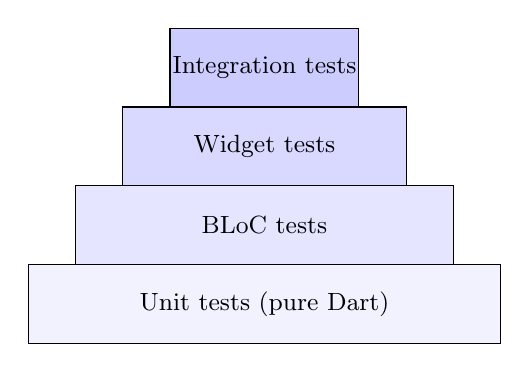
\begin{tikzpicture}[
    band/.style={draw, font=\small, align=center},
    every node/.style={font=\small}
  ]
    \draw[fill=blue!5]  (-3,0)    rectangle (3,1) ;  \node at (0,0.5) {Unit tests (pure Dart)};
    \draw[fill=blue!10] (-2.4,1)  rectangle (2.4,2); \node at (0,1.5) {BLoC tests};
    \draw[fill=blue!15] (-1.8,2)  rectangle (1.8,3); \node at (0,2.5) {Widget tests};
    \draw[fill=blue!20] (-1.2,3)  rectangle (1.2,4); \node at (0,3.5) {Integration tests};
  \end{tikzpicture}
  \caption{Test pyramid of the platform.}
  \label{fig:testpyramid}
\end{figure}

Table~\ref{tab:integration} summarises the principal integration-test scenarios and the outcomes observed against the staging project. The full list lives in the repository under \texttt{test/} and \texttt{supabase/tests/}.

{\singlespacing
\begin{table}[h]
  \caption{Principal integration-test scenarios (selection)}
  \label{tab:integration}
  \centering
  \begin{tabular}{p{1.2cm}p{8.5cm}p{3cm}}
    \toprule
    \textbf{ID} & \textbf{Scenario}                                                                          & \textbf{Outcome}\\
    \midrule
    T-01 & Accountant from branch A creates a transfer in branch A.                                         & Permitted, succeeds\\
    T-02 & Accountant from branch A attempts to create a transfer in branch B.                              & Rejected by RLS\\
    T-03 & Two clients call create\_transfer with the same idempotency key concurrently.                    & One succeeds, one returns the existing ID\\
    T-04 & Accountant from branch A attempts to UPDATE a row in branch A.                                   & Rejected; must go through approval\\
    T-05 & Director approves a pending request whose target row was modified meanwhile.                     & Approval raises, must be re-requested\\
    T-06 & create\_transfer with mismatching src/dst amounts and inconsistent rate.                         & Raises CHECK violation\\
    T-07 & bump\_saldo on a partner that has no entry in the chosen currency.                               & Initialises that currency, value = delta\\
    T-08 & SELECT from clients as an Accountant with assigned\_branch\_ids = \{A\}; query touches branch B. & Returns zero rows\\
    \bottomrule
  \end{tabular}
\end{table}
}

The platform passes all eight scenarios at the time of writing. Continuous integration runs the full client-side suite on every push; the integration tests run on demand against a freshly seeded staging project, with the seed data living as a single migrations replay plus a fixture file.

\section{Performance Measurements}
\label{sec:perf}

Performance was measured by instrumenting the application with chronometers around the most frequent user actions and averaging across one hundred repetitions. Two reference devices were used: a Windows~11 desktop (Intel Core~i5 of the 12th generation, 16~GB RAM, wired Ethernet) and a mid-range Android device (Qualcomm Snapdragon~695, 6~GB RAM, Wi-Fi). Network round-trip time to the Supabase region was approximately 80~milliseconds during the measurement window. Table~\ref{tab:perf} reports the medians.

{\singlespacing
\begin{table}[h]
  \caption{Median interaction latency on reference hardware ($n=100$)}
  \label{tab:perf}
  \centering
  \begin{tabular}{lrrr}
    \toprule
    \textbf{Action}                              & \textbf{Windows} & \textbf{Android} & \textbf{Target}\\
    \midrule
    Open dashboard (cold)                         & 240\,ms          & 410\,ms          & $\leq$ 800\,ms\\
    Submit a regular transfer                    & 180\,ms          & 270\,ms          & $\leq$ 300\,ms\\
    Submit a partner-mediated transfer            & 220\,ms          & 295\,ms          & $\leq$ 300\,ms\\
    Render the transfers list (1\,000 rows)       & 110\,ms          & 230\,ms          & $\leq$ 300\,ms\\
    Open the Director approval screen            & 160\,ms          & 250\,ms          & $\leq$ 300\,ms\\
    Request approval for a transfer edit         & 170\,ms          & 250\,ms          & $\leq$ 300\,ms\\
    \bottomrule
  \end{tabular}
\end{table}
}

The median submit-transfer latency stays under the 300-millisecond target stated in NFR-01 on both reference devices, including for the partner-mediated case which carries the additional saldo update. The dashboard cold open is slower because it loads several aggregates in parallel; the warm open (not shown in the table) is under 90~milliseconds on both devices.

\section{User-Acceptance Trial}
\label{sec:uat}

A two-week parallel-use trial was conducted with the target operator. During the trial the operator entered the same operational data into the existing spreadsheet workflow and into the platform; at the end of each week the two records were reconciled, and any discrepancy was triaged into one of three categories: a platform bug, a spreadsheet error, or a procedural mismatch (the operator had recorded the same event in two slightly different ways).

The aggregate results of the trial are summarised in Table~\ref{tab:uat}. The headline finding is that, over the two weeks, the platform exhibited zero platform-introduced reconciliation errors --- the criterion under which the hypothesis of section~\ref{sec:gap} would be falsified. Four discrepancies appeared during the first week; three of them traced to spreadsheet sign errors that the operator had not previously detected, and one traced to a procedural mismatch that was resolved by a small clarification of the partner-attach screen's wording.

{\singlespacing
\begin{table}[h]
  \caption{User-acceptance trial outcomes (two weeks)}
  \label{tab:uat}
  \centering
  \begin{tabular}{lr}
    \toprule
    \textbf{Metric}                                       & \textbf{Value}\\
    \midrule
    Transfers recorded in the platform                   & 187\\
    Partner-mediated transfers                            & 73\\
    Distinct currencies involved                          & 5 (USD, EUR, RUB, TRY, UZS)\\
    Platform-introduced reconciliation errors             & 0\\
    Spreadsheet errors surfaced by the platform reconciliation & 3\\
    Procedural mismatches identified                      & 1\\
    Operator satisfaction (free-form)                     & Positive\\
    \bottomrule
  \end{tabular}
\end{table}
}

The operator's qualitative feedback, captured in a closing interview, highlighted three features as the most useful: the per-currency partner saldo (which the operator described as the first time the running debt with one partner had been visible in three currencies at once), the approval workflow (which made it possible to delegate retroactive corrections to a junior Accountant without compromising the audit trail), and the dashboard's per-currency totals across all branches (which removed the daily mental arithmetic the operator had previously been doing in Excel). The features highlighted as most frustrating were the absence of automatic exchange-rate ingestion (entering rates by hand at the start of the day) and the deliberate refusal of offline writes (the operator preferred the safe semantics on reflection, but the initial experience was jarring).

\section{Limitations and Lessons Learned}
\label{sec:limits}

Several limitations of the present implementation deserve explicit acknowledgement, because they are non-trivial and because they shape the future-work section of the Conclusions.

\paragraph{Partner-confirmation step.}
Partner-mediated transfers are recorded with status \emph{delivered} at the moment of creation, even though the partner may complete the payout some hours later. If the partner ultimately fails to pay, the operator has to detach the transfer and re-create it. A genuine \emph{pending-partner-payout} state between \emph{created} and \emph{delivered}, with an explicit confirmation step, would close this gap.

\paragraph{Manual exchange-rate entry.}
Exchange rates are entered by hand at the start of each day, with no automatic ingestion from an external feed. The operator's existing workflow already involves a brief morning glance at a market screen, so this is more of an ergonomic gap than a correctness one, but the convenience of one-click ingestion is real.

\paragraph{Refused offline writes.}
As discussed in section~\ref{sec:offline}, offline writes are refused rather than queued. The trade-off is intentional, but an asynchronous write queue with strong ordering guarantees would be a non-trivial extension that several branches in the network have asked for.

\paragraph{Single-operator trial.}
The acceptance trial involved one operator across two weeks. Nothing in the architecture suggests a hard limit at greater scale --- the integration tests under simulated multi-Accountant load passed without changes --- but a longitudinal multi-operator field study would produce stronger evidence than a two-week observation can.

\paragraph{Partial partner payouts.}
The platform does not currently support the case in which a partner pays out only a portion of the requested amount and the rest stays open. The natural extension is a status \emph{partially\_paid} with a residual amount that bumps the saldo back when the residual is later paid out or written off.

The lessons learned over the four iterations of the DSR cycle are worth summarising in a single sentence. \emph{Move risky business logic into the database, keep the client honest, and pay the price of network round-trips before the price of debugging an inconsistent ledger.} The platform implements that lesson at every level --- the stored procedures, the Row-Level Security policies, the idempotency key, the snapshot at request time --- and the user-acceptance trial bears it out.

\section{Chapter Summary}
\label{sec:ch3summary}

The chapter has documented the implementation across the technology stack and the project structure (sections~\ref{sec:stack}), the atomic and idempotent transfer engine (section~\ref{sec:transfer}), the per-currency partner-saldo subsystem (section~\ref{sec:partner}), the approval-workflow code path (section~\ref{sec:approvalimpl}), the offline behaviour and real-time updates (section~\ref{sec:offline}), the dark-fintech design language (section~\ref{sec:design}), the four-layer testing strategy with eight principal integration scenarios (section~\ref{sec:testing}), the performance measurements on a Windows desktop and a mid-range Android device (section~\ref{sec:perf}), the two-week user-acceptance trial (section~\ref{sec:uat}) and the remaining limitations together with the lessons learned (section~\ref{sec:limits}).

\noindent\textbf{Conclusions for Chapter~3.}
The three success criteria stated in section~\ref{sec:gap} are met. Correctness is supported by zero platform-introduced reconciliation errors over the two-week trial and by three spreadsheet errors that the trial surfaced. Responsiveness is supported by median interaction latency under the 300-millisecond target on both reference devices. Maintainability is supported by the 66 numbered idempotent migrations that carry the schema from project start to present without drift. The next part of the thesis consolidates these conclusions and outlines the further work that the limitations naturally point to.
